\documentclass[12pt]{report}
\usepackage[T1]{fontenc}
\usepackage{float}
\usepackage{makeidx}
\usepackage{graphicx} % Required for inserting images
\usepackage{hyperref}
\usepackage[left=2cm, right=2cm]{geometry}
\usepackage[sorting=none]{biblatex}
\usepackage{csquotes}
\usepackage[italian]{babel}
\usepackage{listings}
\lstset{
    basicstyle=\ttfamily,
    showstringspaces=false,
    breaklines=true,
}

\linespread{1}
\addbibresource{pages/bibliography.bib}

\makeindex
\begin{document}
\title{}
\date{}

\begin{titlepage}
    \begin{figure}[t]
        \centering
\includegraphics[width=0.2\textwidth]{images/unibo.jpg}
    \end{figure}
    \begin{center}
        \textsc{ \LARGE{ALMA MATER STUDIORUM - UNIVERSITÀ DI BOLOGNA\\}}
        \textsc{ \Large{Facoltà di INGEGNERIA\\ }}
        \textnormal{ \LARGE{Corso di Laurea Triennale in Ingegneria e Scienze Informatiche\\}}
        \vspace{8mm}
        \fontsize{8mm}{7mm}\selectfont 
        \textup{PROGETTAZIONE DI UN'ARCHITETTURA DI CACHING PER IMMAGINI DOCKER E PACCHETTI LINUX: HARBOR IN MODALITÀ PULL-THROUGH CACHE}\\
    \end{center}
    
    \vspace{8mm}
    
    \begin{minipage}[t]{0.47\textwidth}
        \textnormal{\large{\bf Relatore:\\}}
        {\large Prof. Vittorio Ghini\\}
    \end{minipage}\hfill\begin{minipage}[t]{0.47\textwidth}\raggedleft
        \textnormal{\large{\bf Candidato:\\}}
        {\large Luca Patrignani\\}
    \end{minipage}
    
    
    
    \centering{\large{Sessione II \\ Anno accademico 2023/2024 }}
    
    \end{titlepage}

\maketitle
\tableofcontents

\chapter{Introduzione}
Una organizzazione che fa uso di immagini di container Docker ha bisogno di salvare le immagini che utilizza per i seguenti motivi:
\begin{itemize}
    \item Salvaguardarsi dalla rimozione di alcune immagini dai registry pubblici utili all'organizzazione
    \item Velocizzare il download delle immagini ed impegnare meno banda di rete
    \item Non subire ad ogni pull la limitazione di banda che i registry pubblici (come Docker Hub) impongono agli utenti\cite{hub-rate-limit}.
\end{itemize}
Questo progetto si pone come obiettivo la creazione di un sistema per il caching di immagini docker.

\chapter{Soluzione}
Per risolvere questo problema si è scelto di usare il registry open source Harbor.
\section{Cos'è Harbor}
Harbor\cite{harbor} è una piattaforma open source per la gestione di immagini container che serve come un registro di immagini Docker e OCI (Open Container Initiative) con funzioni avanzate per la sicurezza, la gestione degli utenti e l'amministrazione dei progetti. È progettato per aiutare le organizzazioni a distribuire, proteggere e gestire immagini container nel proprio ambiente di sviluppo e produzione.
\section{Funzionalità principali di Harbor}
\begin{itemize}
    \item \textbf{Registry}: Funziona come un registry Docker, permettendo agli utenti di archiviare, condividere e gestire immagini Docker.
    \item \textbf{Sicurezza}: Harbor integra funzionalità di scansione delle vulnerabilità per identificare problemi di sicurezza nelle immagini container.
    \item \textbf{Gestione dei progetti}: Consente la creazione di progetti privati e pubblici, la gestione degli utenti e la definizione dei permessi di accesso.
    \item \textbf{Replica delle immagini}: Supporta la replica delle immagini tra diversi registri per garantire la disponibilità e la resilienza.
    \item \textbf{Integrazione con Active Directory e LDAP}: Facilita la gestione degli utenti attraverso l'integrazione con servizi di directory aziendali.
    \item \textbf{Audit e Tracciamento}: Fornisce funzionalità di auditing per monitorare le attività e garantire la conformità.
\end{itemize}
Harbor permette la creazione di progetti in modalità proxy cache cioè consente di utilizzare Harbor per fare da proxy e memorizzare nella cache le immagini da un registry pubblico o privato, come ad esempio Docker Hub. È possibile utilizzare un proxy cache per scaricare immagini da un registro Harbor o non-Harbor in un ambiente con accesso limitato o assente a Internet.
\section{Alternative a Harbor}
Due alternative a Harbor sono Nexus di Sonatype e Distribution di Docker.
\subsection{Sonatype Nexus}
Sonatype Nexus è un gestore di repository universale che può ospitare diversi tipi di artefatti, non solo immagini container. È comunemente utilizzato in ambienti aziendali dove è necessario gestire una varietà di artefatti software (ad esempio, librerie Java, pacchetti npm, immagini Docker).
\subsubsection{Caratteristiche principali}
\begin{itemize}
  \item \textbf{Supporto Multi-Formato:} Gestisce diversi tipi di artefatti, incluse immagini Docker, Maven, npm, PyPI, NuGet e altri.
  \item \textbf{Sicurezza e Conformità:} Si integra con Nexus IQ per scansione avanzata delle vulnerabilità, gestione delle licenze e controlli di conformità.
  \item \textbf{Capacità di Registro Docker:} Fornisce un repository Docker per l'hosting e la gestione delle immagini container con funzionalità come controllo degli accessi basato su ruoli e caching.
  \item \textbf{Proxy e Caching dei Repository:} Può fare da proxy a repository esterni e memorizzare localmente gli artefatti in cache per migliorare le prestazioni.
  \item \textbf{Integrazione con CI/CD:} Si integra facilmente con le pipeline CI/CD, permettendo processi di build e deployment fluidi.
  \item \textbf{Funzionalità Enterprise:} Offre alta disponibilità, mirroring dei repository e supporto avanzato, rendendolo adatto per grandi organizzazioni.\cite{nexus}
\end{itemize}
\subsubsection{Casi d'uso}
\begin{itemize}
  \item Organizzazioni che necessitano di un unico strumento di gestione dei repository per diversi tipi di artefatti, non solo immagini Docker.
  \item Aziende alla ricerca di funzionalità avanzate di sicurezza, conformità e gestione degli artefatti.
  \item Team che necessitano di una soluzione robusta e tutto-in-uno che includa capacità di registro Docker accanto ad altri repository.
\end{itemize}

Si è scelto Harbor perché è open source e ci permette di creare diversi progetti nella stessa installazione.

\subsection{Docker Distribution (Docker Registry)}
Docker Distribution comunemente noto come Docker Registry, è lo strumento open source che fornisce le funzionalità di archiviazione e distribuzione per le immagini Docker. È il componente centrale dietro Docker Hub e altri registri Docker. \cite{distribution}

\subsubsection{Caratteristiche principali:}
\begin{itemize}
  \item \textbf{Registro Docker Core:} Fornisce le capacità di base necessarie per archiviare e distribuire immagini Docker.
  \item \textbf{Semplicità e Leggerezza:} Si concentra sull'essere semplice e leggero, adatto per esigenze di hosting e distribuzione di immagini di base.
  \item \textbf{Open Source:} La base per la maggior parte dei registri container, disponibile gratuitamente con licenza open source.
  \item \textbf{Scalabile:} Supporta deployment su larga scala con funzionalità di base, come il supporto per backend di archiviazione (S3, Azure, Google Cloud, ecc.).
  \item \textbf{Caching dei Layer delle Immagini:} Archivia efficientemente le immagini Docker memorizzando in cache i layer, riducendo l'uso di spazio e larghezza di banda.
\end{itemize}

\subsubsection{Casi d'uso}
\begin{itemize}
  \item Team che necessitano di un registro di immagini Docker semplice e leggero.
  \item Organizzazioni che desiderano costruire registri personalizzati o integrare l'archiviazione delle immagini Docker con altri sistemi.
  \item Casi d'uso di base in cui non sono richieste funzionalità avanzate come la scansione di sicurezza, la fiducia del contenuto e il supporto multi-tenant.
\end{itemize}

\section{Come funziona Harbor in modalità cache}
Quando arriva una richiesta di pull a un progetto di proxy cache, se l'immagine non è memorizzata nella cache Harbor recupera l'immagine dal registro di destinazione e soddisfa il comando di pull come se fosse un'immagine locale del progetto di proxy cache. Il progetto di proxy cache quindi memorizza l'immagine nella cache per future richieste.

La prossima volta che un utente richiede quella immagine, Harbor controlla il manifest più recente dell'immagine nel registro target e fornisce l'immagine in base ai seguenti scenari:
\begin{itemize}
    \item Se l'immagine non è stata aggiornata nel registro di destinazione, l'immagine memorizzata nella cache viene servita dal progetto di proxy cache.
    \item Se l'immagine è stata aggiornata nel registro di destinazione, la nuova immagine viene recuperata dal registro di destinazione, quindi servita e memorizzata nella cache nel progetto di proxy cache.
    \item Se il registro di destinazione non è raggiungibile, il progetto di proxy cache serve l'immagine memorizzata nella cache.
    \item Se l'immagine non è più presente nel registro di destinazione, nessuna immagine viene servita. \cite{harbor-pull-through-cache}
\end{itemize}

\chapter{Sicurezza}
\section{Creare un certificato SSL/TLS firmato da una CA}
Harbor, se installato correttamente, accetta richieste https. Ha bisogno però di un certificato digitale emesso da una Certificate Authority. In questo caso si è scelto di utilizzare il protocollo ACME. 
\subsection{Protocollo ACME}
Il protocollo ACME (Automatic Certificate Management Environment)\cite{acme} è uno standard sviluppato per automatizzare l'emissione e la gestione dei certificati digitali, in particolare i certificati SSL/TLS, che sono utilizzati per la crittografia delle comunicazioni su Internet.
Questo è il suo funzionamento di base:
\begin{itemize}
    \item Registrazione: Il client si registra con il server CA, creando un account e ottenendo una coppia di chiavi pubblica/privata.
    \item Richiesta di una sfida: Il client richiede una sfida (challenge) per dimostrare il controllo del dominio. Il protocollo contempla 4 tipi di sfide\cite{acme-challenges}:
    \begin{itemize}
        \item HTTP-01 challenge: La CA ACME richiede al client di ospitare un numero casuale in un URL casuale in \texttt{/.well-known/acme-challenge} sulla porta 80. La CA verifica il controllo del client sul quel dominio e su quella porta riservata emettendo una richiesta HTTP GET a quell'URL.
        \item DNS-01 challenge: La CA ACME richiede al client di configurare un record DNS TXT casuale per il dominio in questione. La verifica della sfida avviene tramite una query DNS per quel record TXT.
        \item TLS-ALPN-01 challenge: La CA ACME utilizza TLS per validare una sfida, sfruttando la negoziazione del protocollo a livello di applicazione (ALPN) durante la TLS handshake. Il client presenta un certificato TLS auto-firmato che contiene la risposta alla sfida come un'estensione speciale del certificato X.509.
        \item DEVICE-ATTEST-01 challenge: progettata per emettere certificati client legati a un identificatore del dispositivo. Permette ai client con un modulo di sicurezza integrato (TPM, Secure Enclave, Yubikey, ecc.) di richiedere un certificato legato all'identificatore hardware permanente del modulo di sicurezza. Può anche essere utilizzata per attestare la protezione hardware di una chiave privata nel modulo di sicurezza.
    \end{itemize}
    \item Risposta alla sfida.
    \item Verifica: La CA verifica che la sfida sia stata completata con successo.
    \item Emissione del certificato: Se la verifica ha esito positivo, la CA emette il certificato, che il client può scaricare e installare.
    \item Rinnovo: ACME automatizza anche il processo di rinnovo del certificato, eseguendo nuovamente le sfide di controllo del dominio prima della scadenza del certificato.
\end{itemize}
Non possiamo però superare nessuna delle sfide: 
\begin{itemize}
    \item HTTP-01: poiché la nostra rete a cui siamo collegati è dietro NAT non abbiamo il controllo sulla porta 80.
    \item DNS-01: non possediamo ne un ip pubblico ne un dominio pubblico per creare un record DNS.
\end{itemize}
Però nel nostro caso non è possibile creare un certificato firmato da una certificate authority pubblica.
Ci si può accontentare di un certificato "self signed" oppure è possibile create una certificate authority all'interno della propria rete privata ed imporre al browser di accettare quei certificati. Nel nostro caso particolare, dove idealmente Harbor è installato "on premise", questa seconda opzione è da preferirsi. Una implementazione open source di una CA è step-ca, sviluppata da Smallstep.
\section{Step-ce e alternative}
In questa sezione, confronteremo tre strumenti comuni per la gestione dei certificati: \textit{step-ca}, \textit{CFSSL} e \textit{Vault} di HashiCorp. Ognuno di questi strumenti ha caratteristiche, casi d'uso e obiettivi differenti.

\subsection{step-ca}
\textit{step-ca} è parte del toolkit di Smallstep, un'autorità di certificazione (CA) open source progettata per semplificare il processo di gestione dei certificati TLS. È pensato per essere facile da usare, soprattutto per i team DevOps che cercano di automatizzare l'emissione, il rinnovo e la gestione dei certificati.

\subsubsection{Caratteristiche principali}:
\begin{itemize}
    \item Semplice da installare e configurare.
    \item Supporta il protocollo ACME (utilizzato da Let's Encrypt).
    \item Ideale per esigenze PKI interne (ad esempio, per emettere certificati per servizi interni, infrastrutture, cluster Kubernetes).
    \item Strumenti moderni e API RESTful.
\end{itemize}

\subsection{CFSSL}
\textit{CFSSL} (CloudFlare's PKI/TLS toolkit) è un altro strumento open source per la gestione di certificati e infrastrutture PKI. È stato sviluppato da Cloudflare e offre una serie di strumenti per la gestione dei certificati, la creazione di una CA, e la gestione di chiavi private.

\subsubsection{Caratteristiche principali}:
\begin{itemize}
    \item Fornisce strumenti per la generazione e la firma di certificati.
    \item Include un servizio di CA API-based che può essere integrato in vari sistemi.
    \item Supporta politiche avanzate di gestione dei certificati.
    \item Adatto per ambienti dove è richiesta una gestione dettagliata e personalizzabile dei certificati.
\end{itemize}

\subsection{Vault di HashiCorp}
\textit{Vault} di HashiCorp è uno strumento di gestione dei segreti che offre anche funzionalità di gestione dei certificati. Vault è progettato principalmente per la gestione sicura di segreti (come API keys, password, certificati, ecc.), ma può fungere anche da CA.

\subsubsection{Caratteristiche principali}:
\begin{itemize}
    \item Gestione centralizzata dei segreti, incluse chiavi API, password e certificati.
    \item Capacità di operare come CA per emettere e rinnovare certificati.
    \item Integrazione con molti sistemi di autenticazione (LDAP, AWS IAM, Kubernetes, ecc.).
    \item Adatto per ambienti complessi che richiedono una gestione avanzata dei segreti e dei certificati.
\end{itemize}
Si è scelto step-ca di Smallstep principalmente per la sua facilità d'uso e il supporto ad ACME.

\chapter{Autenticazione degli utenti}
Harbor permette di integrare servizi di identity provider e usare quegli utenti e gruppi all'interno dei propri progetti. Quindi i dipendenti potranno usare le proprie credenziali aziendali per accedere alla dashboard di Harbor e fare login tramite il comando \texttt{docker login} alle repository a cui hanno il diritto di accedere. Harbor supporta quattro modalità di autenticazione:
\begin{itemize}
    \item Autenticazione tramite database: gli account utente sono creati e gestiti direttamente in Harbor. Gli account utente sono archiviati nel database di Harbor.
    \item Autenticazione tramite LDAP/Active Directory: Harbor è connesso a un server LDAP/Active Directory esterno. Gli account utente vengono creati e gestiti dal provider LDAP/AD.
    \item Autenticazione tramite Provider OIDC: Harbor è connesso a un provider OIDC esterno. Gli account utente vengono creati e gestiti dal provider OIDC.\cite{harbor-auth}
\end{itemize}
Questo livello di sicurezza può risultare ridondante se Harbor è installato all'interno di una rete privata dove l'accesso alla rete stessa dovrebbe garantire un adeguato livello di sicurezza ma di garantire o revocare certi diritti a certi utenti. Per quanto riguarda invece una installazione accessibile da internet (cioè raggiungibile anche da fuori della rete aziendale senza passare per una VPN o altri sistemi di tunnelling) allora diventa di vitale importanza questo livello di autenticazione.
Dato che il caso studio riguarda una azienda è molto probabile che questa abbia già un proprio servizio di active directory che supporti nativamente LDAP, perciò si è deciso di utilizzare questo protocollo.

\section{LDAP}
LDAP (acronimo di Lightweight Directory Access Protocol) è un protocollo open-source e multipiattaforma utilizzato per accedere e gestire directory di informazioni. Una directory in questo contesto è un archivio che contiene dati strutturati gerarchicamente, come una rubrica di contatti o informazioni su utenti, computer e altre risorse di rete.\cite{ldap}
\section{Caratteristiche principali di LDAP}
\begin{itemize}
    \item \textbf{Gestione centralizzata}: LDAP viene utilizzato principalmente per la gestione centralizzata degli utenti e delle risorse. Questo significa che tutte le informazioni sugli utenti (come nomi utente, password, indirizzi email) e le risorse di rete (come stampanti, server) possono essere gestite da un unico punto.
    \item \textbf{Autenticazione e autorizzazione}: LDAP è comunemente utilizzato per autenticare utenti e fornire accesso alle risorse in una rete. Ad esempio, molti sistemi operativi, applicazioni e servizi utilizzano LDAP per verificare le credenziali degli utenti.
    \item \textbf{Interoperabilità}: Essendo un protocollo standard, LDAP è supportato da molti sistemi e applicazioni, rendendolo una scelta popolare per ambienti eterogenei con diverse piattaforme e sistemi operativi.
    \item \textbf{Leggero}: Come suggerisce il nome, LDAP è progettato per essere "leggero" in termini di risorse di rete e di calcolo richieste, rispetto ai protocolli più vecchi e più complessi.
    \item \textbf{Distribuzione e replica}: LDAP supporta la distribuzione dei dati e la replica, permettendo di avere copie dei dati della directory in diverse posizioni, migliorando così la disponibilità e la tolleranza ai guasti.
\end{itemize}
Esiste una versione sicura di LDAP: LDAPS. LDAPS utilizza TLS (Transport Layer Security) o SSL (Secure Sockets Layer) per cifrare la comunicazione tra client e server LDAP, garantendo così che i dati scambiati non possano essere intercettati o modificati da terzi.
\section{Distinguished Name}
Un concetto fondamentale nel protocollo LDAP è quello di \textit{Distinguished Name}. Il DN identifica in modo univoco ogni voce in una directory LDAP.
Il DN è formato da una serie di attributi, ciascuno con un valore, che rappresentano i diversi livelli della struttura della directory. La struttura tipica di un DN può includere (in ordine dal più specifico al più generale):
\begin{itemize}
    \item \textbf{CN (Common Name)}: Nome comune dell'oggetto.
    \item \textbf{OU (Organizational Unit)}: Unità organizzativa.
    \item \textbf{O (Organization)}: Organizzazione.
    \item \textbf{DC (Domain Component)}: Componente di dominio.
    \item \textbf{L (Locality)}: Località.
    \item \textbf{ST (State or Province)}: Stato o provincia.
    \item \textbf{C (Country)}: Paese.\cite{distinguished-name}
\end{itemize}
\subsection{Esempi di DN}
\begin{itemize}
    \item DN di un Utente: \texttt{CN=John Doe,OU=Users,DC=example,DC=com}. Questo DN rappresenta un utente di nome John Doe che è membro dell'unità organizzativa "Users" sotto il dominio "example.com".
    \item DN di un Gruppo: \texttt{CN=Developers,OU=Groups,DC=example,DC=com}. Questo DN rappresenta un gruppo chiamato "Developers" che si trova nell'unità organizzativa "Groups" sotto il dominio "example.com".
\end{itemize}
\subsection{Uso del DN}
\begin{itemize}
    \item Ricerca: Il DN viene utilizzato per localizzare una voce specifica nella directory.
    \item Autenticazione: Il DN può essere usato come parte delle credenziali per autenticare un utente.
    \item Modifica: Le operazioni di modifica su una voce richiedono di specificare il suo DN.
\end{itemize}

\chapter{Installazione Harbor}
Esistono due modalità di Installazione di Harbor: una che usa Docker Compose ed un'altra su Kubernetes. In questo progetto ci si è utilizzata la prima. Ho perciò installato Harbor su una macchina virtuale usando Vagrant. Vagrant è uno strumento open source progettato per creare e gestire ambienti di sviluppo virtualizzati. Vagrant ci permette di fare provisioning della macchina virtuale, cioè mi ha permesso di scrivere uno script che permette l'installazione automatizzata di Harbor e di tutte le sue dipendenze.
\section{Architettura interna di Harbor}
Dalla versione 2.0, Harbor è evoluto diventando un registro di artefatti cloud-native completamente conforme all'OCI.

Un registro di artefatti cloud-native conforme all'OCI significa che ora supporta immagini OCI e indici di immagini OCI (https://github.com/opencontainers/image-spec/blob/master/image-index.md). Un indice di immagini OCI è un manifesto di livello superiore che punta a una lista di manifesti di immagini, ideale per una o più piattaforme. Ad esempio, la lista dei manifesti Docker è un'implementazione popolare dell'indice di immagini OCI. Questo significa anche che Harbor ora supporta pienamente immagini multi-architettura.

Con Harbor V2.0, gli utenti possono gestire immagini, liste di manifesti, Helm charts, CNABs, OPAs, tra gli altri, che aderiscono tutti alle specifiche dell'immagine OCI. Permette inoltre di effettuare operazioni di pull, push, cancellazione, tagging, replicazione e scansione su questo tipo di artefatti. Ora è anche possibile firmare immagini e liste di manifesti.

Il diagramma mostrato di seguito rappresenta l'architettura generale del registro Harbor.

\begin{figure}[h]
\centering
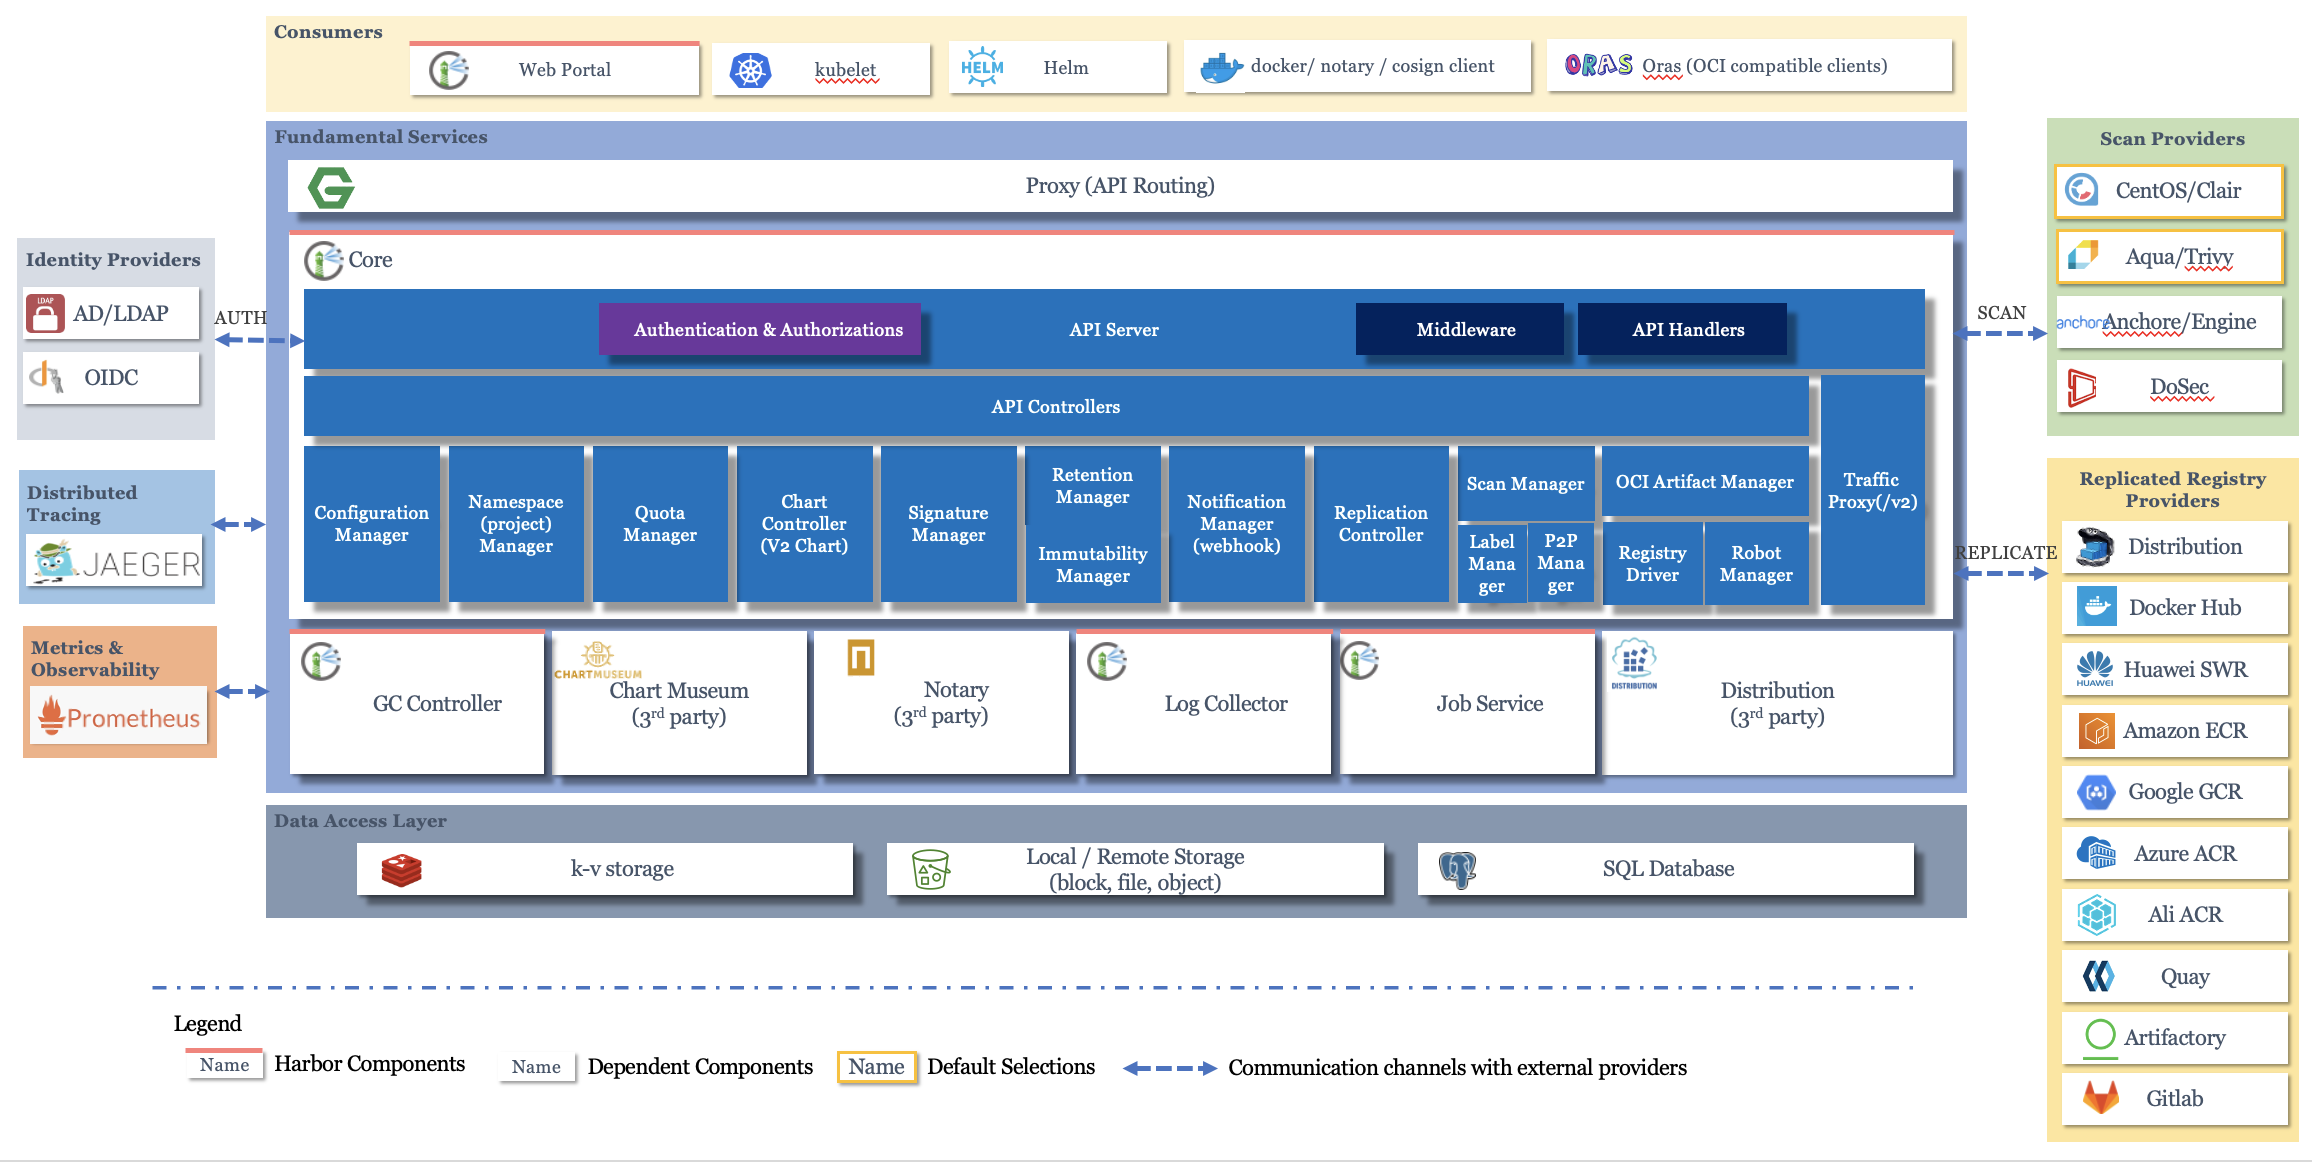
\includegraphics[width=\textwidth]{images/architecture.png}
\caption{Architettura di Harbor versione 2.0.}
\end{figure}

Come rappresentato nel diagramma sopra, Harbor è composto dai seguenti componenti distribuiti su 3 livelli:

\subsection{Livello di Accesso ai Dati}

\textbf{k-v storage}: formato da Redis, fornisce funzioni di cache dei dati e supporta la persistenza temporanea dei metadati dei lavori per il servizio di job.

\textbf{data storage}: diversi tipi di storage sono supportati per la persistenza dei dati come storage di backend del registro e del museo delle chart. Per ulteriori dettagli, fare riferimento al documento della lista dei driver sul sito web di Docker (\url{https://docs.docker.com/registry/storage-drivers/}) e al repository GitHub di ChartMuseum (\url{https://github.com/chartmuseum/storage}).

\textbf{Database}: memorizza i metadati correlati dei modelli di Harbor, come progetti, utenti, ruoli, politiche di replicazione, politiche di conservazione dei tag, scanner, chart e immagini.

\subsection{Servizi principali}

\textbf{Proxy}: reverse-proxy formato dal server Nginx per fornire funzionalità di routing delle API. I componenti di Harbor, come il core, il registro, il portale web e i servizi token, ecc., sono tutti dietro questo proxy inverso. Il proxy inoltra le richieste dai browser e dai client Docker ai vari servizi di backend.

\textbf{Core}: servizio principale di Harbor, che fornisce principalmente le seguenti funzioni:

\begin{itemize}
  \item \textbf{API Server}: un server HTTP che accetta richieste API REST e risponde a queste richieste basandosi sui suoi sottomoduli come 'Autenticazione e Autorizzazione', 'Middleware' e 'Gestori API'.
  \begin{itemize}
    \item \textbf{Autenticazione e Autorizzazione}:
    \begin{itemize}
      \item Le richieste sono protette dal servizio di autenticazione, che può essere gestito da un database locale, AD/LDAP o OIDC.
      \item Il meccanismo RBAC è abilitato per eseguire autorizzazioni sulle azioni correlate, ad esempio: pull/push di un'immagine.
      \item Il servizio token è progettato per emettere un token per ogni comando di push/pull di Docker in base al ruolo dell'utente in un progetto. Se non c'è un token in una richiesta inviata da un client Docker, il Registro reindirizzerà la richiesta al servizio token.
    \end{itemize}
    \item \textbf{Gestori API}: gestiscono le richieste REST API corrispondenti, concentrandosi principalmente sull'analisi e la convalida dei parametri della richiesta, completando la logica aziendale sulla base del controller API pertinente e scrivendo la risposta generata.
  \end{itemize}
  \item \textbf{Config Manager}: copre la gestione di tutte le configurazioni del sistema, come le impostazioni del tipo di autenticazione, le impostazioni email e i certificati, ecc.
  \item \textbf{Gestione dei Progetti}: gestisce i dati di base e i metadati corrispondenti del progetto, che è stato creato per isolare gli artefatti gestiti.
  \item \textbf{Quota Manager}: gestisce le impostazioni delle quote dei progetti ed esegue le convalide delle quote quando avvengono nuovi push.
  \item \textbf{Chart Controller}: fa da proxy per le richieste relative alle chart al backend `chartmuseum` e fornisce diverse estensioni per migliorare l'esperienza di gestione delle chart.
  \item \textbf{Retention Manager}: gestisce le politiche di conservazione dei tag, eseguendo e monitorando i processi di conservazione dei tag.
  \item \textbf{Content Trust}: aggiunge estensioni alla capacità di fiducia fornita dal backend Notary per supportare il processo di fiducia dei contenuti in modo fluido. Al momento, solo le immagini dei container sono supportate per la firma.
  \item \textbf{Replication Controller}: gestisce le politiche di replicazione e gli adattatori del registro, innesca e monitora i processi di replicazione concorrenti. Molti adattatori del registro sono implementati:
  \begin{itemize}
    \item Distribution (docker registry)
    \item Docker Hub
    \item Huawei SWR
    \item Amazon ECR
    \item Google GCR
    \item Azure ACR
    \item Ali ACR
    \item Helm Hub
    \item Quay
    \item Artifactory
    \item GitLab Registry
  \end{itemize}
  \item \textbf{Scan Manager}: gestisce i vari scanner configurati adattati da diversi fornitori e fornisce anche sommari di scansione e report per gli artefatti specificati.
  \item \textbf{Notification Manager (webhook)}: un meccanismo configurato in Harbor in modo che le modifiche di stato degli artefatti in Harbor possano essere popolate agli endpoint Webhook configurati in Harbor. Le parti interessate possono innescare alcune azioni di follow-up ascoltando gli eventi webhook correlati. Attualmente, sono supportati due modi:
  \begin{itemize}
    \item Richiesta HTTP Post
    \item Canale Slack
  \end{itemize}
  \item \textbf{OCI Artifact Manager}: componente core per gestire il ciclo di vita di tutti gli artefatti OCI in tutto il registro Harbor. Fornisce le operazioni CRUD per gestire i metadati e le aggiunte correlate come il report di scansione, la cronologia di costruzione delle immagini del container e il readme, le dipendenze e il valore.yaml delle chart helm, ecc., dell'artefatto, supporta anche le capacità di gestione dei tag degli artefatti e altre operazioni utili.
  \item \textbf{Registry Driver}: implementato come SDK del client del registro per fare comunicazioni con il registro sottostante (distribuzione Docker al momento). 'OCI Artifact Manager' si basa su questo driver per ottenere informazioni aggiuntive dal manifesto e persino dalla configurazione JSON dell'artefatto specificato che si trova nel registro sottostante.
\end{itemize}

\textbf{Servizio di Lavoro}: servizio di coda di esecuzione di lavori generali per permettere ad altri componenti/servizi di inviare richieste per eseguire compiti asincroni in parallelo tramite semplici API REST.

\textbf{Collettore di Log}: raccoglitore di log, responsabile della raccolta dei log degli altri moduli in un unico luogo.

\textbf{Controller di GC}: gestisce le impostazioni del programma GC online e avvia e traccia il progresso del GC.

\textbf{Chart Museum}: un server repository di chart di terze parti che fornisce API di gestione e accesso alle chart. Per maggiori dettagli, consulta \url{https://chartmuseum.com}.

\textbf{Registro Docker}: un server registry di terze parti, responsabile della memorizzazione delle immagini Docker e dell'elaborazione dei comandi push/pull di Docker. Poiché Harbor deve applicare il controllo degli accessi alle immagini, il Registry indirizzerà i client a un servizio token per ottenere un token valido per ogni richiesta di pull o push.

\textbf{Notary}: un server di fiducia del contenuto di terze parti, responsabile della pubblicazione e verifica sicura dei contenuti. Per maggiori dettagli, consulta \url{https://github.com/theupdateframework/notary}.

\subsection{Consumatori}
Come registro standard di artefatti cloud-native, i client correlati saranno naturalmente supportati, come Docker CLI, client Notary, client compatibile OCI come Oras e Helm. Oltre a questi client, Harbor fornisce anche un portale web per consentire agli amministratori di gestire e monitorare facilmente tutti gli artefatti.

\subsection{Il processo di \texttt{docker login}}
Un utente esegue il comando docker per inviare una richiesta di login a Harbor:
\begin{verbatim}
$ docker login https://harbor.domain
\end{verbatim}

Dopo che l'utente inserisce le credenziali richieste, il client Docker invia una richiesta HTTP GET all'indirizzo "https://harbor.domain/v2/". I diversi container di Harbor la processano secondo i seguenti passaggi:
\begin{enumerate}
    \item La richiesta viene ricevuta dal container proxy in ascolto sulla porta 80. Nginx nel container inoltra la richiesta al Registry container sul backend;
    \item Il Registry container è stato configurato per l'autenticazione basata su token, quindi restituisce un codice di errore 401, notificando al client Docker di ottenere un token valido da un URL specificato. In Harbor, questo URL punta al servizio token dei Servizi Core;
    \item Quando il client Docker riceve questo codice di errore, invia una richiesta all'URL del servizio token, incorporando nome utente e password nell'intestazione della richiesta secondo l'autenticazione di base delle specifiche HTTP;
    \item Dopo che questa richiesta è stata inviata al container proxy tramite la porta 80, Nginx inoltra nuovamente la richiesta al container UI secondo le regole preconfigurate. Il servizio token all'interno del container UI riceve la richiesta, la decodifica e ottiene il nome utente e la password;
    \item Dopo aver ottenuto il nome utente e la password, il servizio token controlla il database e autentica l'utente in base ai dati nel database PostgreSQL. Quando il servizio token è configurato per l'autenticazione LDAP/AD, come nel nostro caso, autentica contro il server LDAP/AD esterno. Dopo l'autenticazione riuscita, il servizio token restituisce un codice HTTP che indica il successo. Il corpo della risposta HTTP contiene un token generato da una chiave privata.
\end{enumerate}
A questo punto, un processo di login di docker è stato completato.

\subsection{Il processo di \texttt{docker push}}

Dopo che l'utente ha effettuato con successo l'accesso, un'immagine Docker viene inviata a Harbor tramite il comando:
\begin{verbatim}
# docker push https://harbor.domain/library/hello-world
\end{verbatim}

\begin{enumerate}
    \item In primo luogo, il client docker ripete il processo simile al login inviando la richiesta al registro, e quindi riceve l'URL del servizio token;
    \item Successivamente, quando si contatta il servizio token, il client Docker fornisce informazioni aggiuntive per richiedere un token per l'operazione di push sull'immagine (library/hello-world);
    \item Dopo aver ricevuto la richiesta inoltrata da Nginx, il servizio token interroga il database per verificare il ruolo dell'utente e i permessi per il push dell'immagine. Se l'utente ha il permesso adeguato, codifica le informazioni dell'operazione di push, le firma con una chiave privata e genera un token per il client Docker;
    \item Dopo che il client Docker ottiene il token, invia una richiesta di push al registro con un'intestazione contenente il token. Una volta che il Registro riceve la richiesta, decodifica il token con la chiave pubblica e ne valida il contenuto. La chiave pubblica corrisponde alla chiave privata del servizio token. Se il registro trova il token valido per il push dell'immagine, inizia il processo di trasferimento dell'immagine.\cite{harbor-arch}
\end{enumerate}

\section{Integrazione con la CA}
Poiché è richiesto che Harbor utilizzi https, abbiamo prima bisogno di ottenere un certificato da una CA. È stato perciò usato Certbot, uno utility a riga di comando che permette di ottenere certificati SSL/TLS. Certbot per ottenere tale certificato ha bisogno dei seguenti parametri:
\begin{itemize}
    \item il dominio DNS per cui si richiede il certificato
    \item il server che ospita la CA
    \item un indirizzo email
    \item una flag con cui si dichiara di accettare le condizioni del servizio
\end{itemize}
Inoltre dato che in questo caso è si fa uso di una CA locale e non certificata da una CA fidata bisogna passare a Certbot una variabile di ambiente che contiene il percorso del file che contiene il \texttt{root.ca}, cioè il certificato della nostra CA e che Certbot deve accettare come certificate authority affidabile.
\section{Integrazione con il server LDAP}
Per configurare la modalità di autenticazione di Harbor è stata utilizzata la vastissima RESTful API messa a disposizione. 
Facendo una chiamata PUT all'endpoint \texttt{/api/v2.0/configurations} è possibile configurare Harbor in ogni suo aspetto. La richiesta ha questo aspetto:
\begin{lstlisting}[language=bash]
curl -X PUT -u "<username>:<password>" 
-H "Content-Type: application/json" 
-ki https://<harbor-domain>/api/v2.0/configurations 
-d'{
    "auth_mode": "ldap_auth",
    "ldap_url": "ldap://<ldap-domain>:<ldap-port>",
    "ldap_base_dn": "ou=people,dc=<ldap-domain>",
    "ldap_search_dn": "uid=admin,ou=people,dc=<ldap-domain>",
    "ldap_search_password": "<password>",
    "ldap_group_base_dn": "ou=groups,dc=<ldap-domain>",
    "ldap_group_admin_dn": "cn=<harbor-admin-group>,ou=groups,dc=<ldap-domain>",
    "ldap_group_search_filter": "(objectClass=groupOfUniqueNames)",
    "ldap_group_attribute_name": "uid",
    "ldap_uid": "uid"
}'
\end{lstlisting}
Ecco la spiegazione dei campi più importanti:
\begin{itemize}
    \item \texttt{auth\_mode}: modalità di autenticazione
    \item \texttt{ldap\_url}: l'url del server ldap da utilizzare
    \item \texttt{ldap\_base\_dn}: il Distinguished Name che identifica tutti gli utenti da considerare
    \item \texttt{ldap\_search\_dn}: il DN di un utente che ha diritto di lettura nel server LDAP (il cosiddetto utente bind)
    \item \texttt{ldap\_search\_password}: la password dell'utente bind
    \item \texttt{ldap\_group\_base\_dn}: il gruppo contenente gli utenti che potranno accedere ad Harbor
    \item \texttt{ldap\_group\_admin\_dn}: il gruppo contenente gli utenti che saranno amministratori dell'istanza Harbor
    \item \texttt{ldap\_uid}: l'attributo che gli utenti dovranno inserire come nome utente quando accederanno ad Harbor. \cite{harbor-auth}
\end{itemize}
\section{Domain Name System}
Vagrant ha numerosi plugin, uno di questi è vagrant-dns, che permette la creazione di un server dns che gestisce un dominio locale. Nel Vagrantfile è possibile assegnare un nome di dominio alle macchine virtuali. Questo è fondamentale per il funzionamento di Harbor, infatti Harbor espone tutti i suoi servizi tramite un proxy Nginx il quale per funzionare correttamente deve ricevere richieste con un nome di dominio. Se si fa una GET verso Nginx con un indirizzo ip "nudo", il server risponde con un errore.
L'aver assegnato un nome di dominio alla macchina che ospita Harbor permetterà inoltre di eseguire una installazione Harbor che farà uso di https.
\subsection{Provisioning e vagrant-dns}
Quando un box di Vagrant viene acceso il plugin vagrant-dns crea un nuovo record DNS per quella macchina con il nome di dominio assegnatogli. Per creare uno nuovo record DNS vagrant-dns ha ovviamente bisogno dell'indirizzo ip a cui corrisponderà il nuovo nome di dominio. Per ottenere questa informazione viene eseguito un piccolo script di bash all'interno del box che restituisce l'indirizzo ip. Qui sorge il problema: non è detto che al momento dell'esecuzione dello script le configurazioni di rete siano già avvenute (infatti non è quasi mai il caso). Perciò il plugin ritarda tutte le operazioni aspettando il termine del provisioning della macchina. Ma lo script di provisioning contiene anche i comandi per ottenere il certificato https e questa operazione ha bisogno che la macchina sia raggiungibile anche utilizzando il suo nome di dominio, il quale potrebbe essere ancora non stato assegnato. La soluzione a questo problema è scomporre il processo di start up in due fasi:
\begin{enumerate}
    \item Far partire i box senza eseguire provisioning, obbligando perciò vagrant-dns a ripetere lo script per identificare l'indirizzo ip delle varie macchine
    \begin{lstlisting}[language=bash]
        vagrant up --no-provision
    \end{lstlisting}
    \item Ora che le macchine hanno il loro nome DNS assegnato, fare provisioning delle macchine
    \begin{lstlisting}[language=bash]
        vagrant provision
    \end{lstlisting}
\end{enumerate}

\chapter{Installazione degli altri componenti}
\section{Installazione step-ca}
L'installazione di step-ca è abbastanza lineare, l'unica cosa degna di nota è il far eseguire step-ca come un servizio systemD. La CA durante l'inizializzazione richiede tra i vari campi anche l'indirizzo ip e il nome dns della macchina ospitante. Al termine dell'installazione sarà disponibile il \textit{root certificate}, cioè un certificato "self-signed" dalla stessa CA che la identifica. Il certificato root è solitamente reso affidabile tramite un meccanismo diverso da un certificato, come la distribuzione fisica sicura. Ad esempio, alcuni dei certificati root più conosciuti sono distribuiti nei sistemi operativi dai loro produttori.
Nel nostro caso questo certificato è reso disponibile alle altre macchine virtuali della nostra architettura tramite un volume condiviso.

\section{Installazione LLDAP}
LLDAP è un server di autenticazione leggero che implementa un'interfaccia LDAP semplificata. Questo server è un sistema di gestione utenti che è:
\begin{itemize}
    \item semplice da configurare (senza complicazioni con \texttt{slapd}),
    \item semplice da gestire (interfaccia web user-friendly),
    \item a basso consumo di risorse,
    \item basato su principi consolidati con impostazioni di base predefinite, così non devi comprendere le sottigliezze di LDAP.
\end{itemize}
Per il nostro esperimento si è valutato di non scegliere OpenLDAP poiché è molto laboriosa la sua installazione e nel caso reale il servizio LDAP è già presente all'interno della azienda.
La sua installazione è molto semplice perché esiste l'immagine Docker ufficiale \texttt{lldap/lldap} e tramite delle variabili d'ambiente è possibile configurare il server.
Esiste inoltre un progetto esterno che permette il deployment di LLDAP su un cluster Kubernetes. 

\chapter{Conclusioni}
\section{Architettura completa}
L'architettura ottenuta è schematizzata in questo modo \ref{image:gen-arch}:
\begin{itemize}
    \item Il daemon di Docker (autenticato se necessario) può ottenere da Harbor le immagini presenti nel registry remoto Docker Hub (o altri registri),
    \item Minikube può ottenere le immagini necessarie al funzionamento di Kubernetes da Harbor, il quale fa "mirroring" del registry remoto \texttt{registry.k8s.io}, così come le varie immagini che andranno in esecuzione sul cluster.
    \item Harbor gestisce i propri utenti interfacciandosi con un server che implementa il protocollo LDAP.
    \item Tramite un web browser è possibile accedere al portale di Harbor e anche ad una dashboard di LLDAP.
    \item \texttt{ca.domain} emette certificati per permettere l'uso di https. Tutti gli elementi all'interno della rete locale la riconoscono come Certificate Authority fidata.
\end{itemize}
\begin{figure}[h]
    \centering
    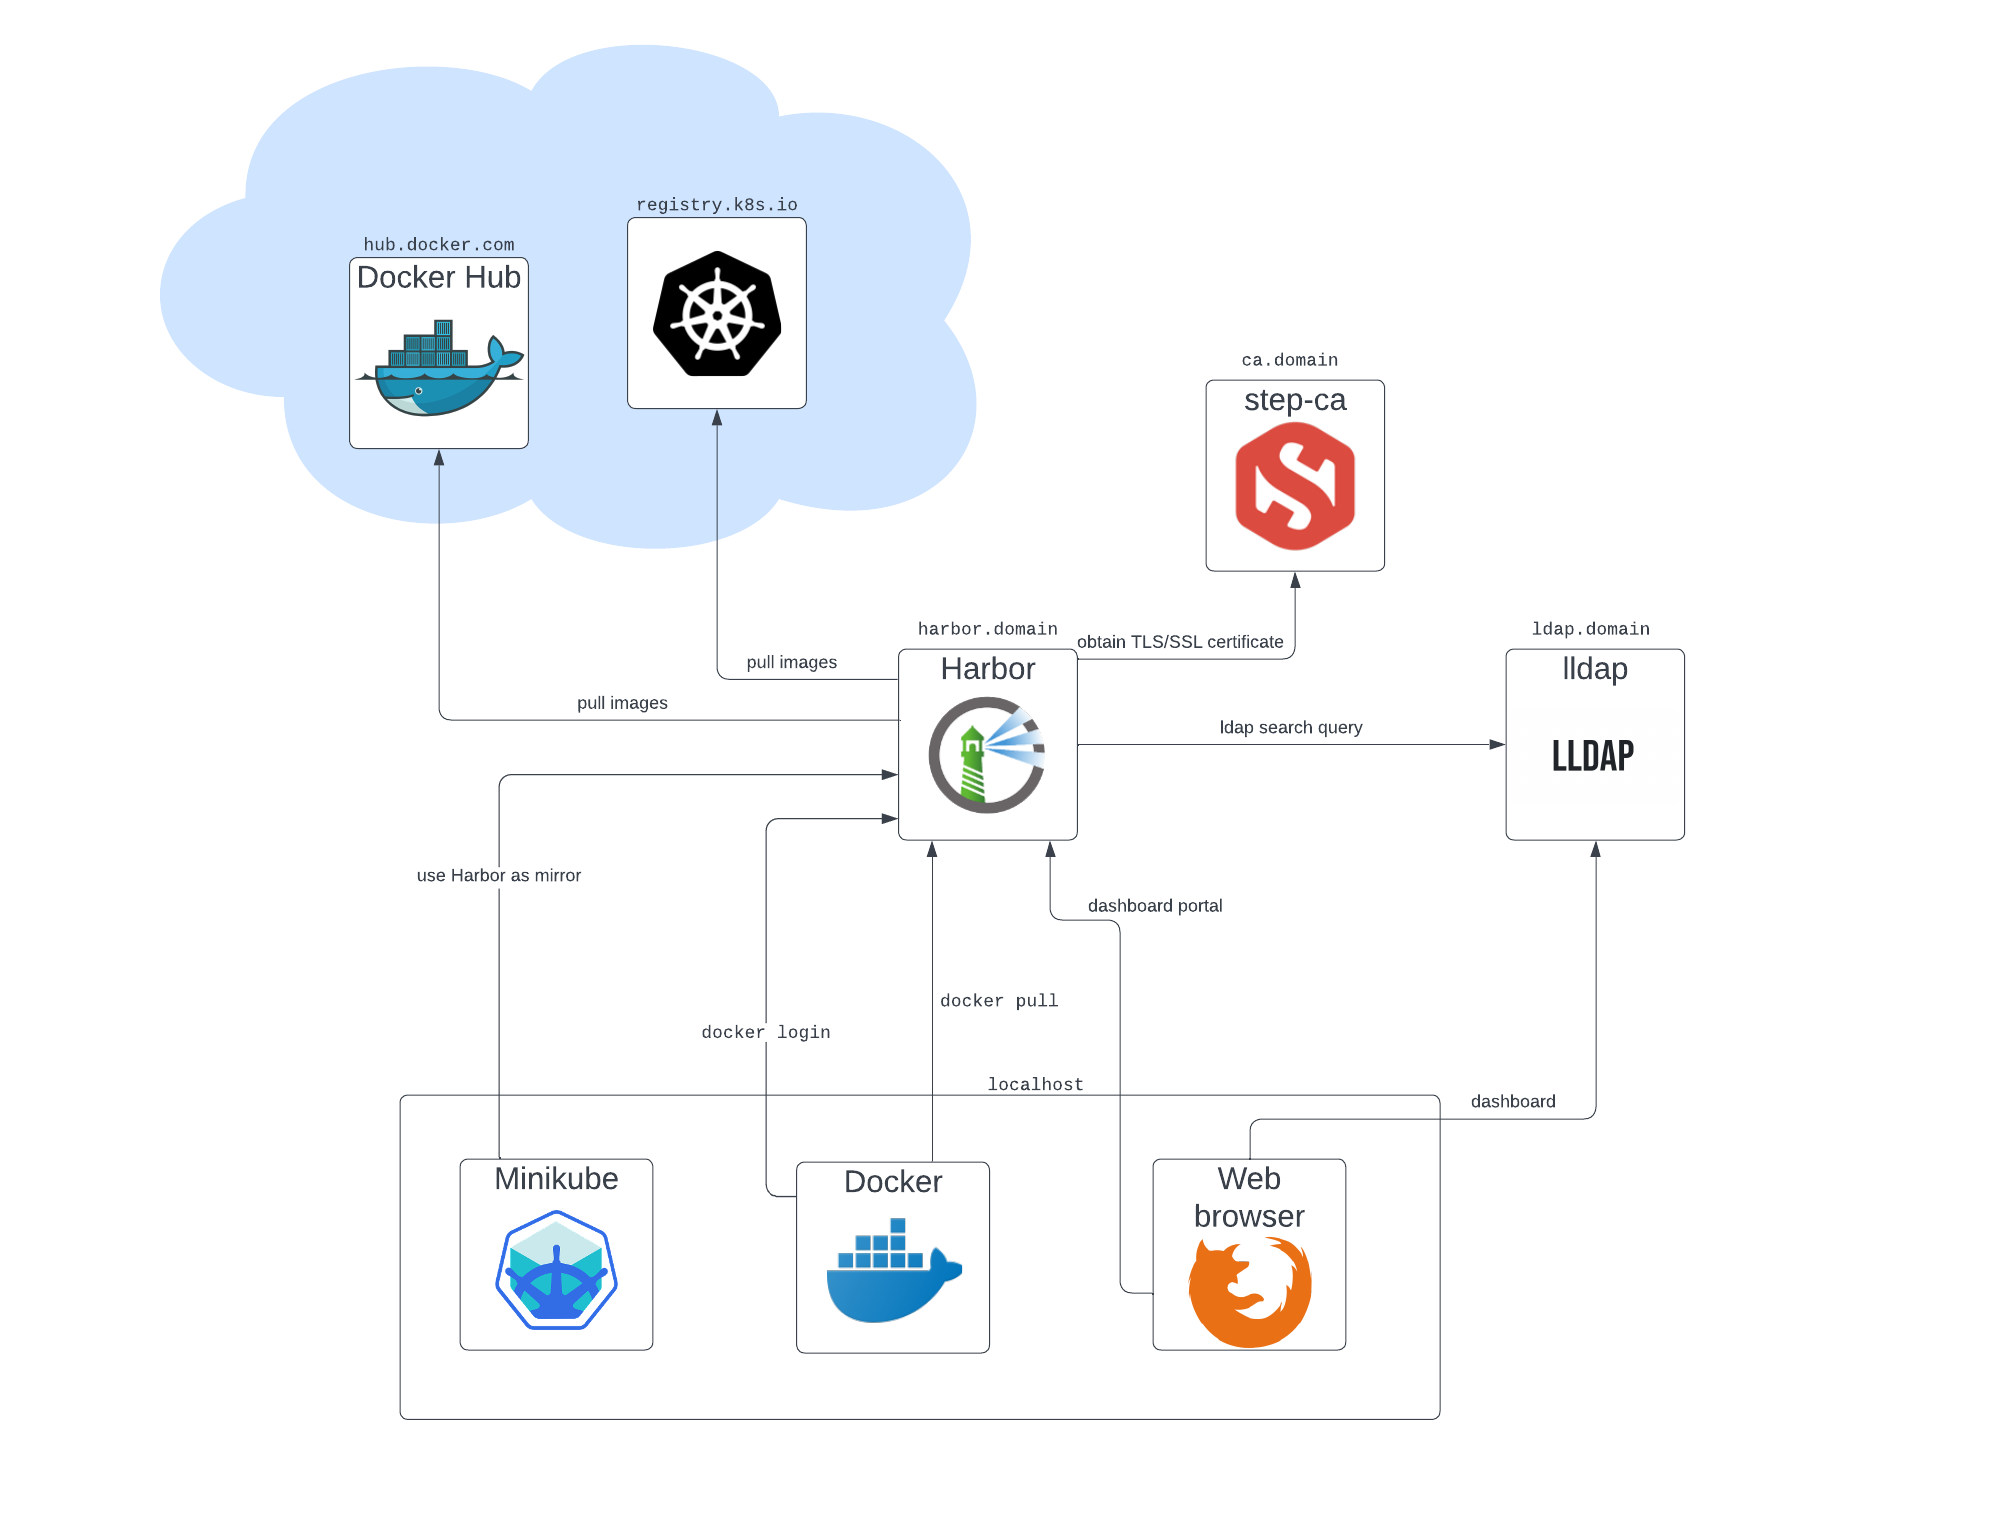
\includegraphics[width=\textwidth]{images/arch-gen.png}
    \caption{Architettura completa del caso studio}
    \label{image:gen-arch}
\end{figure}
\section{Benchmark}
Per mostrare il miglioramento delle prestazioni nella fase di download delle immagini usando la cache che questo progetto di tesi ha creato si è proceduto a scrivere uno script di testing. Lo script prende come argomento il nome di una immagine Docker \texttt{image} presente sul registro pubblico di Docker Hub e restituisce queste misurazioni:
\begin{enumerate}
    \item La dimensione dell'immagine \texttt{image}, colonna Dimensione;
    \item Il tempo in secondi impiegato dal daemon Docker per scaricare una certa immagine \texttt{image} direttamente da Docker Hub, colonna No cache;
    \item Il tempo in secondi impiegato dal daemon Docker per scaricare una certa immagine \texttt{image} da un progetto di Harbor in modalità cache della stessa immagine \textit{non presente} nel progetto, colonna Cache miss;
    \item Il tempo in secondi impiegato dal daemon Docker per scaricare una certa immagine \texttt{image} da un progetto di Harbor in modalità cache della stessa immagine \textit{già presente} nel progetto, colonna Cache hit.
\end{enumerate}
Ecco delle misurazioni effettuate su alcune immagini di esempio, tutte le misurazioni sono state svolte su una installazione locale di Harbor \ref{table:benchmark}.
\begin{table}[]
    \begin{tabular}{|c|c|c|c|c|}
    \hline
                         & \textbf{Dimensione} & \textbf{No cache} & \textbf{Cache miss} & \textbf{Cache hit} \\ \hline
    \textbf{hello-world} & 13,3 kB             & 3,14 s            & 5,35 s              & 0,65 s             \\ \hline
    \textbf{alpine}      & 7.8 MB              & 7,13 s            & 7,08 s              & 1,66 s             \\ \hline
    \textbf{ubuntu}      & 78,1 MB             & 18,78 s           & 26,74 s             & 2,71 s             \\ \hline
    \textbf{fedora}      & 222 MB              & 56,38 s           & 105,31 s            & 4,35 s             \\ \hline
    \textbf{postgres}    & 432 MB              & 92,87 s           & 110,03 s            & 8,82 s             \\ \hline
    \textbf{mysql}       & 586 MB              & 98,77 s           & 191,78 s            & 7,74 s             \\ \hline
    \end{tabular}
    \caption{Tabella che mostra i risultati di alcune misurazioni fatte su un campione di immagini Docker.}
    \label{table:benchmark}
\end{table}
Prima di analizzare questi dati bisogna ricordare che
\begin{itemize}
    \item Le misurazioni variano dalla posizione geografica dell'installazione di Harbor (in questo caso locale)
    \item Le misurazioni variano dalla posizione geografica del server che ci offre le immagini docker (in questo caso Docker Hub)
    \item Le misurazioni variano al variare della banda disponibile durante il download.
\end{itemize}
Detto ciò si può notare come tutti i tempi misurati aumentano all'aumentare della dimensione dell'immagine scaricata, inoltre si nota come i tempi aumentano leggermente quando si ha un cache miss e si riducono notevolmente quando si ha un cache hit.

\printbibliography[heading=bibintoc, title={Bibliografia}]
\end{document}.
